\documentclass[a4paper]{article}

\usepackage[a4paper]{geometry}
\geometry{verbose,tmargin=1.5cm,bmargin=1.5cm,lmargin=1.5cm,rmargin=1.5cm}

\setlength{\parskip}{\smallskipamount}
\setlength{\parindent}{0pt}

\usepackage{fontspec}
\setmonofont{FreeMono}

\usepackage{hyperref}
\usepackage{url}
\usepackage{xcolor}

\usepackage{amsmath}
\usepackage{amssymb}

\usepackage{graphicx}
\usepackage{float}

\usepackage{minted}
\newminted{julia}{breaklines,fontsize=\small}
\newminted{bash}{breaklines,fontsize=\small}
\newminted{text}{breaklines,fontsize=\small}

\newcommand{\txtinline}[1]{\mintinline{text}{#1}}
\newcommand{\jlinline}[1]{\mintinline{julia}{#1}}

\newmintedfile[juliafile]{julia}{breaklines,fontsize=\small}

\definecolor{mintedbg}{rgb}{0.90,0.90,0.90}
\usepackage{mdframed}

\BeforeBeginEnvironment{minted}{\begin{mdframed}[backgroundcolor=mintedbg]}
\AfterEndEnvironment{minted}{\end{mdframed}}

\begin{document}

\title{TF4062: Implementing Density Functional Theory using Finite Difference Method}
\author{Iwan Prasetyo \\
Fadjar Fathurrahman}
\date{}
\maketitle


\section{Introduction}

Density functional theory: \cite{Hohenberg1964,Kohn1965},

Applications: \cite{VanMourik2014}

Books: \cite{Martin2004,Kohanoff2006,Marx2009}

Kohn-Sham equations:
\begin{equation}
\hat{H}_{\mathrm{KS}}\,\psi_{i}(\mathbf{r}) = \epsilon_{i}\,\psi_{i}(\mathbf{r})
\end{equation}

Roadmap of the article:

\section{Schroedinger equation in 1d}

We are interested in finding bound states solution to 1d time-independent Schroedinger equation:
\begin{equation}
\left[ -\frac{1}{2}\frac{\mathrm{d}^2}{\mathrm{d}x^2} + V(x) \right] \psi(x) = E\, \psi(x)
\label{eq:Sch_1d_eq}
\end{equation}
%
with the boundary conditions:
%
\begin{equation}
\lim_{x \rightarrow \pm \infty} \psi(x) = 0
\label{eq:BC_isolated}
\end{equation}
%
First we need to define a spatial domain $\left[x_{\mathrm{min}}, x_{\mathrm{max}}\right]$
where $x_{\mathrm{min}}, x_{\mathrm{max}}$ chosen
such that the boundary condition \ref{eq:BC_isolated} is approximately satisfied.
The next step is to divide the spatial domain $x$ using equally-spaced grid points
which we will denote as $\{x_{1},x_{2},\ldots,x_{N}\}$ where $N$ is number
of grid points. Various spatial quantities such as wave function and potential will be discretized
on these grid points.
The grid points $x_{i}$, $i = 1, 2, \ldots$ are chosen as:
\begin{equation}
x_{i} = x_{\mathrm{min}} + (i-1)h
\end{equation}
where $h$ is the spacing between the grid points:
\begin{equation}
h = \frac{ x_{\mathrm{max}} - x_{\mathrm{min}} }{N-1}
\end{equation}

The following code can be used to initialize the grid points:
\begin{juliacode}
function init_FD1d_grid( x_min::Float64, x_max::Float64, N::Int64 )
    L = x_max - x_min
    h = L/(N-1) # spacing
    x = zeros(Float64,N) # the grid points
    for i = 1:N
        x[i] = x_min + (i-1)*h
    end
    return x, h
end
\end{juliacode}


Approximating second derivative

Our next task is to find an approximation to the second derivative operator
present in the Equation \eqref{eq:Sch_1d_eq}.
One simple approximation that we can use is the 3-point (central) finite difference:
\begin{equation}
\frac{\mathrm{d}^2}{\mathrm{d}x^2} \psi_{i} =
\frac{\psi_{i+1} - 2\psi_{i} + \psi_{i-1}}{h^2}
\end{equation}
where we have the following notation have been used: $\psi_{i} = \psi(x_{i})$.
%
By taking $\{ \psi_{i} \}$ as a column vector, the second derivative operation
can be expressed as matrix multiplication:
\begin{equation}
\vec{\psi''} = \mathbb{D}^{(2)} \vec{\psi}
\end{equation}
%%
where $\mathbb{D}^{(2)}$ is the second derivative matrix operator:
\begin{equation}
\mathbb{D}^{(2)} = \frac{1}{h^2}
\begin{bmatrix}
-2  &  1  &  0  &  0  & 0 & \cdots & 0 \\
 1  & -2  &  1  &  0  & 0 & \cdots & 0 \\
 0  &  1  & -2  &  1  & 0 & \cdots & 0 \\
 \vdots  &  \ddots  &  \ddots  & \ddots  & \ddots  & \ddots & \vdots \\
 0 & \cdots & 0 & 1 & -2 & 1 & 0 \\
 0  &  \cdots  & \cdots & 0  & 1  & -2  & 1 \\
 0  &  \cdots  & \cdots & \cdots & 0  &  1  & -2 \\
\end{bmatrix}
\label{eq:1d_D2_matmul}
\end{equation}

An example implementation can be found in the following function.
\begin{juliacode}
function build_D2_matrix_3pt( N::Int64, h::Float64 )
    mat = zeros(Float64,N,N)
    for i = 1:N-1
        mat[i,i] = -2.0
        mat[i,i+1] = 1.0
        mat[i+1,i] = mat[i,i+1]
    end
    mat[N,N] = -2.0
    return mat/h^2
end
\end{juliacode}


Before use this function to solve Schroedinger equation we will to test the operation
in Equation \eqref{eq:1d_D2_matmul} for a simple function which second derivative
can be calculated analytically.
\begin{equation}
\psi(x) = \mathrm{e}^{-\alpha x^2}
\end{equation}
%
which second derivative can be calculated as
%
\begin{equation}
\psi''(x) = \left( -2 \alpha + 4\alpha^2 x^2 \right) \mathrm{e}^{-\alpha x^2}
\end{equation}
%
They are implemented in the following code
\begin{juliacode}
function my_gaussian(x; α=1.0)
    return exp(-α*x^2)
end

function d2_my_gaussian(x; α=1.0)
    return (-2*α + 4*α^2 * x^2) * exp(-α*x^2)
end
\end{juliacode}

\begin{figure}[H]
{\center
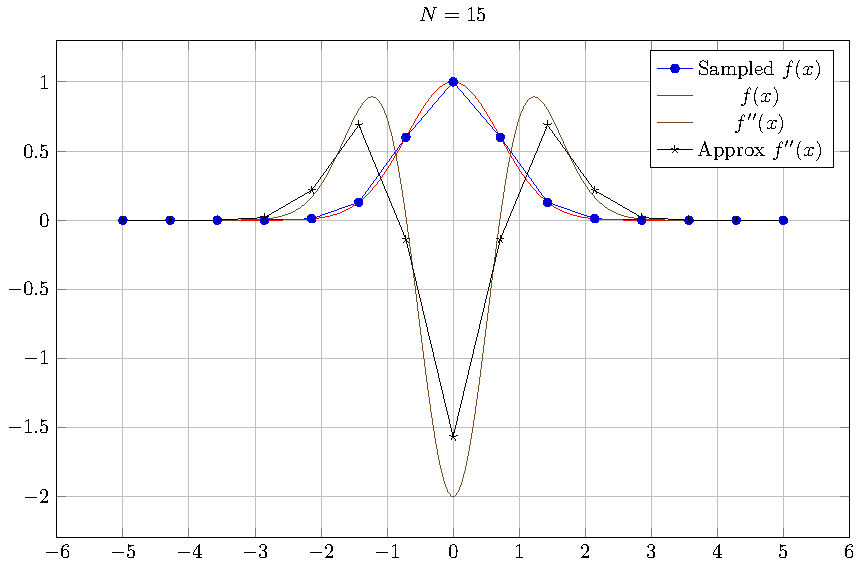
\includegraphics[scale=0.75]{../codes/IMG_gaussian_15.pdf}
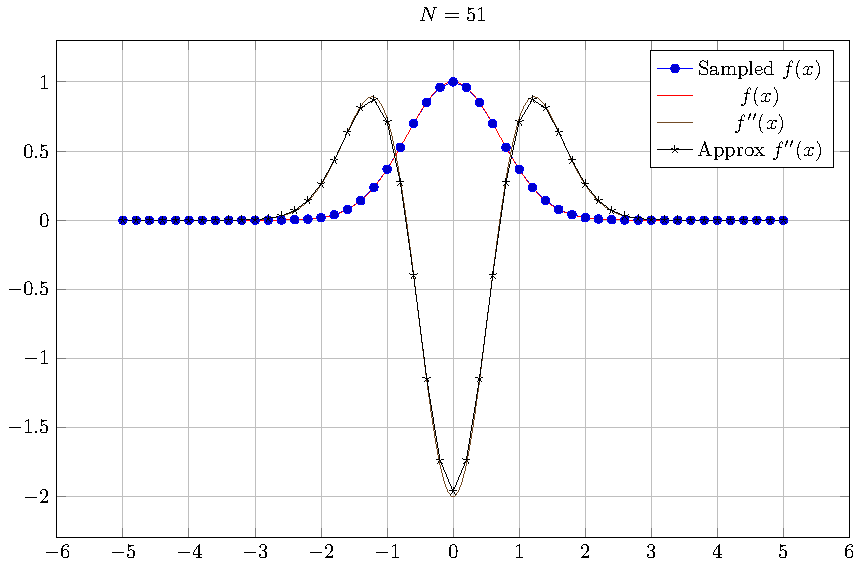
\includegraphics[scale=0.75]{../codes/IMG_gaussian_51.pdf}
\par}
\caption{Finite difference approximation to a Gaussian function and its second derivative}
\end{figure}


Harmonic potential

We will start with a simple potential with known exact solution, namely the harmonic potential:
\begin{equation}
V(x) = \frac{1}{2}\omega^2 x^2
\end{equation}

The Hamiltonian in finite difference representation:
\begin{equation}
\mathbb{H} = -\frac{1}{2}\mathbb{D}^{(2)} + \mathbb{V}
\end{equation}
where $\mathbb{V}$ is a diagonal matrix whose elements are:
\begin{equation}
\mathbb{V}_{ij} = V(x_{i})\delta_{ij}
\end{equation}


Code to solve harmonic oscillator:

\juliafile{../codes/main_harmonic_01.jl}

Compare with analytical solution.

Plot of eigenfunctions:

\begin{figure}[H]
{\center
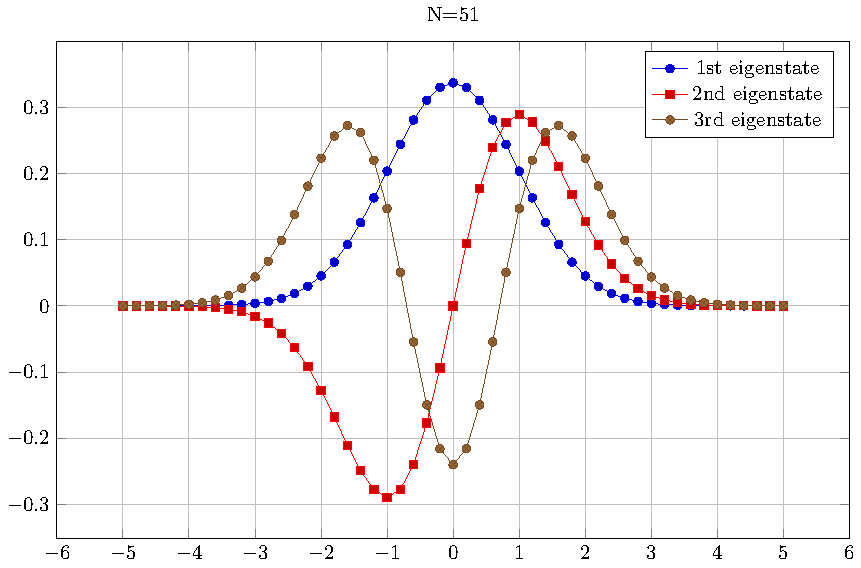
\includegraphics[scale=0.75]{../codes/IMG_main_harmonic_01_51.pdf}
\par}
\caption{Eigenstates of harmonic oscillator}
\end{figure}


\subsection{Higher order finite difference}

An alternative to using more grid points
To obtain higher accuracy

Implementing higher order finite difference.

\section{Schroedinger equation in 2d}

Now we will turn out attention to higher dimensions, i.e 2d.
The Schrodinger equation in 2d reads:
\begin{equation}
\left[ -\frac{1}{2}\nabla^2 + V(x,y) \right] \psi(x,y) = E\,\psi(x,y)
\label{eq:sch_2d}
\end{equation}
%
where $\nabla^2$ is the Laplacian operator:
\begin{equation}
\nabla^2 = \frac{\partial^2}{\partial x^2} + \frac{\partial^2}{\partial y^2}
\end{equation}

\subsection{Describing grid in 2d}

Now we have two directions $x$ and $y$. Our approach to solving the Schroedinger equation
is similar to the one we have used before in 1d, however several technical difficulties
will arise.

To describe the computational grid, we now need to specify $x_{\mathrm{max}}, x_{\mathrm{min}}$ for the X-domain
and $y_{\mathrm{max}}, y_{\mathrm{min}}$ for Y-domain. We also need to specify number of grid
points in for each x and y-directions, i.e. $N_{x}$ and $N_{y}$. That are quite lot of variables.
For easier management, we will collect our grid related variables in one data structure or
\txtinline{struct} in Julia. A \txtinline{struct} in Julia looks very much like C-struct.
It also defines a new custom data type in Julia.

Our struct definition looks like this.
\begin{juliacode}
struct FD2dGrid
    Npoints::Int64
    Nx::Int64
    Ny::Int64
    hx::Float64
    hy::Float64
    dA::Float64
    x::Array{Float64,1}
    y::Array{Float64,1}
    r::Array{Float64,2}
    idx_ip2xy::Array{Int64,2}
    idx_xy2ip::Array{Int64,2}
end
\end{juliacode}
%
An instance of \txtinline{FD2dGrid} can be initialized using the following constructor function:
%
\begin{juliacode}
function FD2dGrid( x_domain, Nx, y_domain, Ny )
    x, hx = init_FD1d_grid(x_domain, Nx)
    y, hy = init_FD1d_grid(y_domain, Ny)
    dA = hx*hy
    Npoints = Nx*Ny
    r = zeros(2,Npoints)
    ip = 0
    idx_ip2xy = zeros(Int64,2,Npoints)
    idx_xy2ip = zeros(Int64,Nx,Ny)
    for j in 1:Ny
        for i in 1:Nx
            ip = ip + 1
            r[1,ip] = x[i]
            r[2,ip] = y[j]
            idx_ip2xy[1,ip] = i
            idx_ip2xy[2,ip] = j
            idx_xy2ip[i,j] = ip
        end
    end
    return FD2dGrid(Npoints, Nx, Ny, hx, hy, dA, x, y, r, idx_ip2xy, idx_xy2ip) 
end
\end{juliacode}

A short explanation about the members of \txtinline{FD2dGrid} follows.
%
\begin{itemize}
%
\item \txtinline{Npoints} is the total number of grid points.
%
\item \txtinline{Nx} and \txtinline{Ny} is the total number of grid points
in $x$ and $y$-directions, respectively.
%
\item \txtinline{hx} and \txtinline{hy} is grid spacing in $x$ and $y$-directions,
respectively. \txtinline{dA} is the product of \txtinline{hx} and \txtinline{hy}.
%
\item \txtinline{x} and \txtinline{y} are the grid points in $x$ and $y$-directions.
The actual two dimensional grid points $r \equiv (x_{i},y_{i})$ are stored as
two dimensional array $r$.
%
\item Thw two integers arrays \txtinline{idx_ip2xy} and \txtinline{idx_xy2ip} defines
mapping between two dimensional grids and linear grids.
\end{itemize}


As an illustration let's build a grid for a rectangular domain
$x_\mathrm{min} = y_{\mathrm{min}}=-5$ and $x_\mathrm{max} = y_{\mathrm{max}}=5$
and $N_{x}=3$, $N_{y}=4$.
Using the above constructor for \txtinline{FD2dGrid}:
\begin{juliacode}
Nx = 3
Ny = 4
fdgrid = FD2dGrid( (-5.0,5.0), Nx, (-5.0,5.0), Ny )
\end{juliacode}
%
Dividing the $x$ and $y$ accordingly we obtain $N_{x}=3$
grid points along $x$-direction
%
\begin{textcode}
> println(fdgrid.x)
[-5.0, 0.0, 5.0]
\end{textcode}
%
and $N_{y}=4$ points along the $y$-direction
\begin{textcode}
> println(fdgrid.y)
[-5.0, -1.6666666666666665, 1.666666666666667, 5.0]
\end{textcode}
%
The actual grid points are stored in \txtinline{fdgrid.r}. Using the
following snippet, we can printout all of the grid points:
%
\begin{juliacode}
for ip = 1:fdgrid.Npoints
    @printf("%3d %8.3f %8.3f\n", ip, fdgrid.r[1,ip], fdgrid.r[2,ip])
end
\end{juliacode}
%
The results are:
%
\begin{textcode}
  1   -5.000   -5.000
  2    0.000   -5.000
  3    5.000   -5.000
  4   -5.000   -1.667
  5    0.000   -1.667
  6    5.000   -1.667
  7   -5.000    1.667
  8    0.000    1.667
  9    5.000    1.667
 10   -5.000    5.000
 11    0.000    5.000
 12    5.000    5.000
\end{textcode}
%
We also can use the usual rearrange these points in the usual 2d grid rearrangement:
%
\begin{textcode}
[  -5.000,  -5.000] [  -5.000,  -1.667] [  -5.000,   1.667] [  -5.000,   5.000] 
[   0.000,  -5.000] [   0.000,  -1.667] [   0.000,   1.667] [   0.000,   5.000] 
[   5.000,  -5.000] [   5.000,  -1.667] [   5.000,   1.667] [   5.000,   5.000]
\end{textcode}
%
which can be produced from the following snippet:
%
\begin{juliacode}
for i = 1:Nx
    for j = 1:Ny
        ip = fdgrid.idx_xy2ip[i,j]
        @printf("[%8.3f,%8.3f] ", fdgrid.r[1,ip], fdgrid.r[2,ip])
    end
    @printf("\n")
end
\end{juliacode}



\subsection{Laplacian operator}

Having built out 2d grid, we now turn our attention to the second derivative operator or
the Laplacian in the equation \ref{eq:sch_2d}.
There are several ways to build a matrix representation of the Laplacian, but we will
use the easiest one. 

Before constructing the Laplacian matrix, there is an important observation that
we should make about the second derivative matrix $\mathbb{D}^{(2)}$. We should note
that the second derivative matrix contains mostly zeros. This type of matrix that
most of its elements are zeros is called \textbf{sparse matrix}.
In a sparse matrix data structure, we only store its non-zero elements with specific
formats such as compressed sparse row/column format (CSR/CSC) and coordinate format.
We have not made use of the sparsity of the second derivative matrix
in the 1d case for simplicity. In the higher dimensions, however,
we must make use of this sparsity, otherwise we will waste computational resources 
by storing many zeros. The Laplacian matrix that we will build from
$\mathbb{D}^{(2)}$ is also very sparse.

Given second derivative matrix in $x$, $\mathbb{D}^{(2)}_{x}$,
$y$ direction, $\mathbb{D}^{(2)}_{x}$,
we can construct finite difference representation of the Laplacian operator
$\mathbb{L}$ by using
%
\begin{equation}
\mathbb{L} = \mathbb{D}^{(2)}_{x} \otimes \mathbb{I}_{y} +
\mathbb{I}_{x} \otimes \mathbb{D}^{(2)}_{y}
\end{equation}
%
where $\otimes$ is Kronecker product.
In Julia, we can use the function \jlinline{kron} to form the Kronecker product
between two matrices \jlinline{A} and \jlinline{B} as \jlinline{kron(A,B)}.

The following function illustrates the above approach to construct matrix
representation of the Laplacian operator.
\begin{juliacode}
function build_nabla2_matrix( fdgrid::FD2dGrid; func_1d=build_D2_matrix_3pt )
    Nx = fdgrid.Nx
    hx = fdgrid.hx
    Ny = fdgrid.Ny
    hy = fdgrid.hy
    
    D2x = func_1d(Nx, hx)
    D2y = func_1d(Ny, hy)

    ∇² = kron(D2x, speye(Ny)) + kron(speye(Nx), D2y)
    return ∇²
end
\end{juliacode}

In the Figure \ref{fig:fd_gaussian_2d}, an example to the approximation of 2nd derivative
of 2d Gaussian function by using finite difference is shown.

\begin{figure}[H]
{\center
\includegraphics[width=0.45\textwidth]{../codes/FD2d/IMG_gaussian2d.pdf}\,%
\includegraphics[width=0.45\textwidth]{../codes/FD2d/IMG_d2_gaussian2d.pdf}
\par}
\caption{Two-dimensional Gaussian function and its finite difference
approximation of second derivative}
\label{fig:fd_gaussian_2d}
\end{figure}

\subsection{Iterative methods for eigenvalue problem}

Now that we know how to build the Laplacian matrix, we now can build the Hamiltonian
matrix given some potential:
\begin{juliacode}
∇² = build_nabla2_matrix( fdgrid )
Ham = -0.5*∇² + spdiagm( 0 => Vpot )
\end{juliacode}
Note that we have used sparse diagonal matrix for building the potential matrix by
using the function \txtinline{spdiagm}.
Our next task after building the Hamiltonian matrix is to find the eigenvalues
and eigenfunctions.
However, note that the Hamiltonian matrix size is large.
For example, if we use $N_x=50$ and $N_y=50$ we will end up with a Hamiltonian
matrix with the size of $2500$.
The use \txtinline{eigen} method to solve this eigenvalue problem is thus not practical.
Actually, given enough computer memory and time, we can use the function
\txtinline{eigen} anyway
to find the eigenvalue and eigenfunction of the Hamiltonian, however it is not recommended
nor practical for larger problem size.

Typically, we also do not need to solve for all eigenvalue and eigenfunction pairs.
We only need to solve for several eigenpairs with lowest eigenvalues. In typical density
functional theory calculations, we typically solve for $N_{\mathrm{electrons}}$ or
$N_{\mathrm{electrons}}/2$ lowest states, where $N_{\mathrm{electrons}}$ is the number
of electrons in the system.

In numerical methods, there are several methods to search for several eigenpairs
of a matrix. These methods falls into the category of \textit{partial or iterative
diagonalization methods}. Several known methods are Lanczos method, Davidson method,
preconditioned conjugate gradients, etc.

In this short article, we will not discuss about these methods in depth.
However, we have prepared several implementation of iterative diagonalization methods
for your convenience:
\begin{itemize}
\item \txtinline{diag_Emin_PCG}
\item \txtinline{diag_davidson}
\item \txtinline{diag_LOBPCG}
\end{itemize}

Almost all iterative methods need a good preconditioner to function properly. In this
talk, we will use several preconditioners that have been implemented in several packages
in Julia such as incomplete LU and multigrid preconditioners.

Here we show an example of Julia program to solve the Schroedinger equation for two
dimensional harmonic potentials. The complete program can be found in the
\txtinline{sch_2d/main_harmonic.jl}.

\begin{juliacode}
function pot_harmonic( fdgrid::FD2dGrid; ω=1.0 )
    Npoints = fdgrid.Npoints
    Vpot = zeros(Npoints)
    for i in 1:Npoints
        x = fdgrid.r[1,i]
        y = fdgrid.r[2,i]
        Vpot[i] = 0.5 * ω^2 *( x^2 + y^2 )
    end
    return Vpot
end

function main()
    Nx = 50
    Ny = 50
    fdgrid = FD2dGrid( (-5.0,5.0), Nx, (-5.0,5.0), Ny )
    ∇2 = build_nabla2_matrix( fdgrid )
    Vpot = pot_harmonic( fdgrid )
    Ham = -0.5*∇2 + spdiagm( 0 => Vpot )

    # Preconditioner based on inverse kinetic
    prec = ilu(-0.5*∇2)

    Nstates = 10
    Npoints = Nx*Ny
    X = rand(Float64, Npoints, Nstates)
    ortho_sqrt!(X)
    
    evals = diag_LOBPCG!( Ham, X, prec, verbose=true )
    X = X/sqrt(fdgrid.dA) # renormalize the eigenfunctions

    @printf("\n\nEigenvalues\n")
    for i in 1:Nstates
        @printf("%5d %18.10f\n", i, evals[i])
    end
end
\end{juliacode}


The eigenfunctions are shown in Figure \ref{fig:harm_2d_eigenfunctions}.

\begin{figure}[H]
{\centering
\includegraphics[scale=0.3]{../codes/sch_2d/IMG_harmonic_psi_1.pdf}\\
\includegraphics[scale=0.3]{../codes/sch_2d/IMG_harmonic_psi_2.pdf}%
\includegraphics[scale=0.3]{../codes/sch_2d/IMG_harmonic_psi_3.pdf}\\
\includegraphics[scale=0.3]{../codes/sch_2d/IMG_harmonic_psi_4.pdf}%
\includegraphics[scale=0.3]{../codes/sch_2d/IMG_harmonic_psi_5.pdf}%
\includegraphics[scale=0.3]{../codes/sch_2d/IMG_harmonic_psi_6.pdf}\\
\includegraphics[scale=0.3]{../codes/sch_2d/IMG_harmonic_psi_7.pdf}%
\includegraphics[scale=0.3]{../codes/sch_2d/IMG_harmonic_psi_8.pdf}%
\includegraphics[scale=0.3]{../codes/sch_2d/IMG_harmonic_psi_9.pdf}%
\includegraphics[scale=0.3]{../codes/sch_2d/IMG_harmonic_psi_10.pdf}
\par}
\label{fig:harm_2d_eigenfunctions}
\end{figure}

Eigenvalues ($N_{x} = N_{y} = 50$):
\begin{textcode}
    1       0.9999999862
    2       1.9999998768
    3       1.9999999392
    4       2.9999992436
    5       2.9999993054
    6       2.9999997845
    7       3.9999973668
    8       3.9999976649
    9       3.9999992565
   10       3.9999998030
\end{textcode}


Energy
\begin{textcode}
n_x + n_y + 1  &  Values of n_x and n_y
1              &  (0,0)
2              &  (1,0) (0,1)
3              &  (2,0) (1,1) (1,1)
4              &  (3,0) (0,3) (2,1) (1,2)
\end{textcode}

Energy:
\begin{equation}
E_{n_{x} + n_{y}} = \hbar \omega \left( n_{x} + n_{y} + 1 \right)
\end{equation}

\section{Schroedinger equation in 3d}

The 3d case of Schroedinger equation is a straightforward extension of the 2d case.
The Schroedinger equation thus reads:
\begin{equation}
\left[ -\frac{1}{2}\nabla^2 + V(x,y,z) \right] \psi(x,y,z) = E\,\psi(x,y,z)
\label{eq:sch_3d}
\end{equation}
%
where $\nabla^2$ is the Laplacian operator:
\begin{equation}
\nabla^2 = \frac{\partial^2}{\partial x^2} + \frac{\partial^2}{\partial y^2} + \frac{\partial^2}{\partial z^2}
\end{equation}

We begin by defining a struct called \txtinline{FD3dGrid} which is a
straightforward generalization of \txtinline{FD2dGrid}. The implementation of this
struct can be found in the file \txtinline{FD3d/FD3dGrid.jl}.

The Lagrangian operator in 3d also can be implemented by straightforward extension
of 2d case.
\begin{juliacode}
const ⊗ = kron

function build_nabla2_matrix( fdgrid::FD3dGrid; func_1d=build_D2_matrix_3pt )

    D2x = func_1d(fdgrid.Nx, fdgrid.hx)
    D2y = func_1d(fdgrid.Ny, fdgrid.hy)
    D2z = func_1d(fdgrid.Nz, fdgrid.hz)

    IIx = speye(fdgrid.Nx)
    IIy = speye(fdgrid.Ny)
    IIz = speye(fdgrid.Nz)

    ∇² = D2x⊗IIy⊗IIz + IIx⊗D2y⊗IIz + IIx⊗IIy⊗D2z 

    return ∇²
end
\end{juliacode}

The main difference is that we have used the symbol \txtinline{⊗} in place
of \txtinline{kron} function to make our code simpler.

We hope that at this point you will have no difficulties to create your own
3d Schroedinger equation solver.

Analytic solution for energy:
\begin{equation}
E_{n_{x} + n_{y} + n_{z}} = \hbar \omega \left( n_{x} + n_{y} + n_{z} + \frac{3}{2} \right)
\end{equation}

Degeneracies:
\begin{equation}
g_{n} = \frac{(n + 1)(n + 2)}{2}
\end{equation}

\begin{textcode}
n = n_x + n_y + n_z

n = 0: (1)(2)/2 = 1
n = 1: (2)(3)/2 = 3
n = 2: (3)(4)/2 = 6
\end{textcode}

\subsection{Hydrogen atom and an introduction to pseudopotential}

Until now, we only have considered simple potentials such as harmonic potential. Now we will
move on and consider more realistic potentials which is used in practical electronic calculations.

For most applications in materials physics and chemistry the external potential that is
felt by electrons is the Coulombic potential due to atomic nucleus. This potential has
the following form:
\begin{equation}
V(r) = -\sum_{I}^{N_{\mathrm{atom}}} \frac{Z_{I}}{\left|\mathbf{r} - \mathbf{R}_{I}\right|}
\end{equation}
where $R_{I}$ are the positions and $Z_{I}$ are the charges
of the atomic nucleus present in the system.
%
We will consider the most simplest system, namely the hydrogen atom $Z_{I}=1$, for which we have
\begin{equation}
V(r) = -\frac{1}{\left|\mathbf{r} - \mathbf{R}_{0}\right|}
\end{equation}
%
The following Julia code implement the H atom potential:
\begin{juliacode}
function pot_H_atom( fdgrid::FD3dGrid; r0=(0.0, 0.0, 0.0) )
    Npoints = fdgrid.Npoints
    Vpot = zeros(Npoints)
    for i in 1:Npoints
        dx = fdgrid.r[1,i] - r0[1]
        dy = fdgrid.r[2,i] - r0[2]
        dz = fdgrid.r[3,i] - r0[3]
        Vpot[i] = -1.0/sqrt(dx^2 + dy^2 + dz^2)
    end
    return Vpot
end
\end{juliacode}

With only minor modification to our program for harmonic potential, we can solve the Schroedinger
equation for the hydrogen atom:
\begin{juliacode}
fdgrid = FD3dGrid( (-5.0,5.0), Nx, (-5.0,5.0), Ny, (-5.0,5.0), Nz )
∇2 = build_nabla2_matrix( fdgrid, func_1d=build_D2_matrix_9pt )
Vpot = pot_H_atom( fdgrid )
Ham = -0.5*∇2 + spdiagm( 0 => Vpot )
prec = aspreconditioner(ruge_stuben(Ham))
Nstates = 1  # only choose the lowest lying state
Npoints = Nx*Ny*Nz
X = ortho_sqrt( rand(Float64, Npoints, Nstates) ) # random initial guess of wave function
evals = diag_LOBPCG!( Ham, X, prec, verbose=true )
\end{juliacode}

For the grid size of $N_{x}=N_{y}=N_{z}=50$ and using 9-point finite-difference approximation
to the second derivative operator in 1d we obtain the eigenvalue of -0.4900670759 Ha which
is not too bad if compared with the exact value of -0.5 Ha. We can try to increase the grid
size until we can get satisfactory result.

Note that there is a caveat when we are trying to use the Coulombic potential. This potential
is diverget at $r=0$, so care must be taken such that this divergence is not encountered in
our potential. We have tried to achieve this by using choosing the numbers
$N_{x}$, $N_{y}$, and $N_{z}$ to be even numbers. This way, we have avoiding encountering
divergence in the calculation of Coulomb potential.

In the many electronic structure calculations, it is sometime convenient to replace the
Coulomb potential with another potential which is smoother which we
will refer to as a \textbf{pseudopotential}. Not all smooth
potentials can do the job. The smooth potential should satisfy several requirements.
One of the most important requirement is that the smooth potential should have similar
scattering properties as the original Coulomb potential that it replaces.
This means that the potential should have posses similar eigenvalues as the
original Coulomb potential. Usually we don't try to reproduce all eigenvalue spectrum but only
the eigenvalues which belongs to the valence electrons. The valence electrons are
responsible for most chemically and physically important properties so this is an
acceptable approximation for most cases.

The theory and algorithms for constructing pseudopotentials are beyond the scope of
this article.
Most pseudopotentials are non-local by construction and this can make our program rather
complicated.
In this article we focus on the so-called local pseudopotential. Practically, local
pseudopotentials pose no additional difficulties as the potentials that we have
considered so far. As an example of a pseudopotential, we will consider the following
local pseudopotential for hydrogen atom:
\begin{equation}
V_{\mathrm{H,ps}}(r) = -\frac{Z_{\mathrm{val}}}{r}
\mathrm{erf}\left( \frac{\bar{r}}{\sqrt{2}} \right) +
\exp\left( -\frac{1}{2}\bar{r}^2 \right)
\left( C_{1} + C_{2}\bar{r}^2 \right)
\end{equation}
where $\bar{r}=r/r_{\mathrm{loc}}$ and with the parameters $r_{loc}=0.2$, 
$Z_{\mathrm{val}}=1$, $C_{1}=-4.0663326$, and $C_{2}=0.6678322$.

\begin{figure}[H]
{\centering
\includegraphics[scale=0.5]{../codes/sch_3d/IMG_H_Coulomb_vs_pspot.pdf}
\par}
\end{figure}

The code
\begin{juliacode}
function pot_Hps_HGH( fdgrid::FD3dGrid; r0=(0.0, 0.0, 0.0) )
    Npoints = fdgrid.Npoints
    Vpot = zeros( Float64, Npoints )

    # Parameters
    Zval = 1
    rloc = 0.2
    C1 = -4.0663326
    C2 = 0.6678322
    for ip = 1:Npoints
        dx2 = ( fdgrid.r[1,ip] - r0[1] )^2
        dy2 = ( fdgrid.r[2,ip] - r0[2] )^2
        dz2 = ( fdgrid.r[3,ip] - r0[3] )^2
        r = sqrt(dx2 + dy2 + dz2)
        if r < eps()
            Vpot[ip] = -2*Zval/(sqrt(2*pi)*rloc) + C1
        else
            rrloc = r/rloc
            Vpot[ip] = -Zval/r * erf( r/(sqrt(2.0)*rloc) ) +
                     (C1 + C2*rrloc^2)*exp(-0.5*(rrloc)^2)
        end
    end
    return Vpot
end
\end{juliacode}



\appendix

\section{Alternative solutions}

\begin{juliacode}
function my_func()
    println("OK ...")
end
\end{juliacode}


\end{document}